\hypertarget{a00847}{}\section{Change Log}
\label{a00847}\index{Change Log@{Change Log}}
Changes between A\+AX S\+DK versions. 

\hypertarget{a00847_changelog}{}\subsection{Change Log}\label{a00847_changelog}
\hypertarget{a00847_aax_sdk_2p3p2}{}\subsubsection{A\+A\+X S\+D\+K 2.\+3.\+2}\label{a00847_aax_sdk_2p3p2}
\hypertarget{a00847_aax_sdk_2p3p2_AAXLibrary}{}\paragraph{A\+A\+X Library}\label{a00847_aax_sdk_2p3p2_AAXLibrary}

\begin{DoxyItemize}
\item Removed unnecessary {\ttfamily virtual} keyword usage for method overrides  
\item Removed unused {\ttfamily m\+Clipped} member of \mbox{\hyperlink{a01481}{A\+A\+X\+\_\+\+C\+Effect\+Parameters}}  
\item Convert {\ttfamily m\+View\+Container} member of \mbox{\hyperlink{a01477}{A\+A\+X\+\_\+\+C\+Effect\+G\+UI}} to a smart pointer  
\end{DoxyItemize}\hypertarget{a00847_aax_sdk_2p3p2_Build}{}\paragraph{Build}\label{a00847_aax_sdk_2p3p2_Build}

\begin{DoxyItemize}
\item Xcode 10 and Visual Studio 2017 are now supported  
\item Added Xcode workspace and Visual Studio solution containing all projects in the A\+AX S\+DK for convenience  
\item Removed 32-\/bit architecture targets from all project configurations. 32-\/bit architectures are still supported by A\+AX if you choose to explicitly add them to your build project configurations.  
\item Updated all Xcode projects to recommended {\ttfamily C\+F\+Bundle\+Identifier} usage and build settings  
\end{DoxyItemize}\hypertarget{a00847_aax_sdk_2p3p2_Definitions}{}\paragraph{Definitions}\label{a00847_aax_sdk_2p3p2_Definitions}

\begin{DoxyItemize}
\item Added \mbox{\hyperlink{a00662_a13e384f22825afd3db6d68395b79ce0da80bb55dbba6cba01120eda8f86284eba}{A\+A\+X\+\_\+e\+Property\+\_\+\+Constraint\+\_\+\+Do\+Not\+Apply\+Default\+Settings}} for plug-\/ins which need to disable the normal default settings application procedure used by Pro Tools  
\item Added \mbox{\hyperlink{a00491_afab5ea2cfd731fc8f163b6caa685406ea40644990a3de0fec1f25929b535f7760}{A\+A\+X\+\_\+e\+Notification\+Event\+\_\+\+Prior\+Settings\+Invalid}} which may be useful for certain plug-\/ins when running in Venue systems  
\item Added \mbox{\hyperlink{a00662_a13e384f22825afd3db6d68395b79ce0da699fa67ab37a566fbcb8fe08d6a3cf8b}{A\+A\+X\+\_\+e\+Property\+\_\+\+Plug\+In\+I\+D\+\_\+\+No\+Processing}} for Effect types that do not process audio  
\item Removed {\ttfamily A\+A\+X\+\_\+e\+Property\+\_\+\+Supports\+Progress\+Dialog} which is not supported in any A\+AX host  
\end{DoxyItemize}\hypertarget{a00847_aax_sdk_2p3p2_Documentation}{}\paragraph{Documentation}\label{a00847_aax_sdk_2p3p2_Documentation}

\begin{DoxyItemize}
\item Fixes and improvements in the \char`\"{}\+Plug-\/\+In spec properties\char`\"{} section of \mbox{\hyperlink{a00662}{A\+A\+X\+\_\+\+Properties.\+h}}  
\item Added \mbox{\hyperlink{a00794_aax_sdk_guide_quickstart}{Quick Start}} and \mbox{\hyperlink{a00842}{Troubleshooting}} documentation sections  
\item Added additional detail to the \mbox{\hyperlink{a00830_subsection__digital_signature_}{Digital signature}} section of the \mbox{\hyperlink{a00830}{Pro Tools Guide}}  
\end{DoxyItemize}\hypertarget{a00847_aax_sdk_2p3p2_ExamplePlugIns}{}\paragraph{Example plug-\/ins}\label{a00847_aax_sdk_2p3p2_ExamplePlugIns}

\begin{DoxyItemize}
\item Changed ID generation algorithm for \mbox{\hyperlink{a00848_DemoGain_UpMixer}{Demo\+Gain\+\_\+\+Up\+Mixer}}. Older copies of this example plug-\/in will not be recovered in saved sessions.  
\end{DoxyItemize}\hypertarget{a00847_aax_sdk_2p3p2_ResolvedBugs}{}\paragraph{Resolved bugs}\label{a00847_aax_sdk_2p3p2_ResolvedBugs}

\begin{DoxyItemize}
\item Fixed \mbox{\hyperlink{a00846_AAXSDK-663}{A\+A\+X\+S\+D\+K-\/663}} A\+AX S\+DK {\ttfamily \#pragma pack} errors with X\+Code 10 and later  
\end{DoxyItemize}\hypertarget{a00847_aax_sdk_2p3p1}{}\subsubsection{A\+A\+X S\+D\+K 2.\+3.\+1}\label{a00847_aax_sdk_2p3p1}
\hypertarget{a00847_aax_sdk_2p3p1_AAXLibrary}{}\paragraph{A\+A\+X Library}\label{a00847_aax_sdk_2p3p1_AAXLibrary}

\begin{DoxyItemize}
\item Enhanced support for \mbox{\hyperlink{a01601}{A\+A\+X\+\_\+\+Checked\+Result}} -\/ added \mbox{\hyperlink{a00497_af9972551e4546e894010f99eade68c94}{A\+A\+X\+\_\+\+C\+A\+P\+T\+U\+RE}}, \mbox{\hyperlink{a00497_a078be92d3d19a5a4b3da2b55ae5ac1c9}{A\+A\+X\+\_\+\+C\+A\+P\+T\+U\+R\+E\+\_\+\+M\+U\+LT}}, and \mbox{\hyperlink{a01605}{A\+A\+X\+\_\+\+Aggregate\+Result}} to assist with common Describe error handling scenarios  
\item Updated \mbox{\hyperlink{a01969_a69f9b80a70ecc6b7b2a7eec372d2502a}{A\+A\+X\+\_\+\+C\+Monolithic\+Parameters\+::\+Static\+Describe()}} to use \mbox{\hyperlink{a01601}{A\+A\+X\+\_\+\+Checked\+Result}} for error checking  
\item Added \mbox{\hyperlink{a01541}{A\+A\+X\+\_\+\+C\+Stateless\+Parameter}} for \char`\"{}momentary\char`\"{} parameters which do not require state, such as tap tempo buttons which can be mapped to a control surface  
\item Improved tolerance for unknown parameters when building or parsing plug-\/in settings chunk data  
\item Added \mbox{\hyperlink{a00395_aa0253bd2994036fcfd6629ecf465d543}{A\+A\+X\+\_\+\+D\+E\+B\+U\+G\+A\+S\+S\+E\+RT}}, \mbox{\hyperlink{a00395_ae871829dd7297e4a5ae6c7094f6b5398}{A\+A\+X\+\_\+\+S\+T\+A\+C\+K\+T\+R\+A\+CE}}, and \mbox{\hyperlink{a00395_a96862f9cb28b6a49eb5dbd6da9975ed1}{A\+A\+X\+\_\+\+T\+R\+A\+C\+E\+O\+R\+S\+T\+A\+C\+K\+T\+R\+A\+CE}} to the library of tracing and assertion macros in \mbox{\hyperlink{a00395}{A\+A\+X\+\_\+\+Assert.\+h}}  
\item Fixed warnings which would prevent compilation in Visual Studio 2015 and Visual Studio 2017 when Treat Warnings As Errors is enabled  
\item Removed Visual Studio 2008, Visual Studio 2010, and Xcode 3 projects  
\end{DoxyItemize}\hypertarget{a00847_aax_sdk_2p3p1_Definitions}{}\paragraph{Definitions}\label{a00847_aax_sdk_2p3p1_Definitions}

\begin{DoxyItemize}
\item Removed guard preventing \mbox{\hyperlink{a00392_a2da185ff8aad77278f985a6fe5ee07ba}{A\+A\+X\+\_\+\+C\+P\+P11\+\_\+\+S\+U\+P\+P\+O\+RT}} from being set for P\+A\+CE Fusion compiler builds  
\item Deprecated \mbox{\hyperlink{a00491_af7d77416967955e258539694870f395a}{A\+A\+X\+\_\+\+E\+Host\+Mode}} -\/ replaced by \mbox{\hyperlink{a00491_aa3c8056a6ce601cc3367cb7d4478e9da}{A\+A\+X\+\_\+\+E\+Host\+Mode\+Bits}}  
\end{DoxyItemize}\hypertarget{a00847_aax_sdk_2p3p1_Documentation}{}\paragraph{Documentation}\label{a00847_aax_sdk_2p3p1_Documentation}

\begin{DoxyItemize}
\item Documentation added to \mbox{\hyperlink{a00812}{EQ and Dynamics Curve Displays}} for the EQ Curves feature in Pro Tools 2018.\+1  
\item Added \mbox{\hyperlink{a00796_describe_checking_results}{Checking Results}} and \mbox{\hyperlink{a00796_describe_validation}{Describe Validation}} sections to \mbox{\hyperlink{a00796}{Description callback}}  
\item Added \mbox{\hyperlink{a00843_aax_distributing_installer}{Building your plug-\/in installer}} section to \mbox{\hyperlink{a00843}{Distributing Your A\+AX Plug-\/\+In}}, including information about bundling Track Presets with the plug-\/in installer  
\end{DoxyItemize}\hypertarget{a00847_aax_sdk_2p3p1_ExamplePlugIns}{}\paragraph{Example plug-\/ins}\label{a00847_aax_sdk_2p3p1_ExamplePlugIns}

\begin{DoxyItemize}
\item Updated all example plug-\/ins\textquotesingle{} Describe routines to use \mbox{\hyperlink{a01601}{A\+A\+X\+\_\+\+Checked\+Result}} for error checking  
\item Updated some example plug-\/ins\textquotesingle{} parameter registration code in \mbox{\hyperlink{a01481_a2e302fd758d39a6a855023bf825fe148}{Effect\+Init()}} with a safer parameter creation and release style using std\+::unique\+\_\+ptr  
\item Updated the \mbox{\hyperlink{a00848_RectiFi}{Recti\+Fi}} example plug-\/in to match the current shipping version of Avid\textquotesingle{}s Recti-\/\+Fi plug-\/in  
\item \mbox{\hyperlink{a00848_DemoGain_UpMixer}{Demo\+Gain\+\_\+\+Up\+Mixer}} now converts arbitrarily between all stem formats, both wider and narrower  
\item Removed Visual Studio 2008, Visual Studio 2010, and Xcode 3 projects  
\item Common Xcode settings updated with \char`\"{}macosx10.\+11\char`\"{} base S\+DK and \char`\"{}10.\+9\char`\"{} deployment target  
\item Added \mbox{\hyperlink{a00852}{A\+AX}} D\+SP for higher stem formats in \mbox{\hyperlink{a00848_DemoGain_Multichannel}{Demo\+Gain\+\_\+\+Multichannel}} and \mbox{\hyperlink{a00848_DemoGain_UpMixer}{Demo\+Gain\+\_\+\+Up\+Mixer}}  
\end{DoxyItemize}\hypertarget{a00847_aax_sdk_2p3p1_Extensions}{}\paragraph{Extensions}\label{a00847_aax_sdk_2p3p1_Extensions}

\begin{DoxyItemize}
\item Updated the V\+S\+T\+G\+UI extension and example plug-\/in to use V\+S\+T\+G\+UI 4.\+3  
\end{DoxyItemize}\hypertarget{a00847_aax_sdk_2p3p1_Interface}{}\paragraph{Interface}\label{a00847_aax_sdk_2p3p1_Interface}

\begin{DoxyItemize}
\item New interfaces\+: 
\begin{DoxyItemize}
\item \mbox{\hyperlink{a01729}{A\+A\+X\+\_\+\+I\+A\+C\+F\+Page\+Table\+\_\+\+V2}}, with methods accessed through \mbox{\hyperlink{a01849}{A\+A\+X\+\_\+\+I\+Page\+Table}} 
\item \mbox{\hyperlink{a01721}{A\+A\+X\+\_\+\+I\+A\+C\+F\+Host\+Services\+\_\+\+V3}}, with methods typically accessed through the macros in \mbox{\hyperlink{a00395}{A\+A\+X\+\_\+\+Assert.\+h}} 
\end{DoxyItemize}See \mbox{\hyperlink{a00845}{Host Support}} for host support information  
\end{DoxyItemize}\hypertarget{a00847_aax_sdk_2p3p1_Utilities}{}\paragraph{Utilities}\label{a00847_aax_sdk_2p3p1_Utilities}

\begin{DoxyItemize}
\item Added reference count tracing logic to A\+A\+X\+\_\+\+C\+A\+C\+F\+Unknown.\+cpp, which can be toggled on using the {\ttfamily A\+A\+X\+\_\+\+D\+E\+B\+U\+G\+\_\+\+A\+C\+F\+\_\+\+R\+E\+F\+C\+O\+U\+NT} macro  
\item Added some convenience functions to \mbox{\hyperlink{a00650}{A\+A\+X\+\_\+\+Page\+Table\+Utilities.\+h}}  
\item Added \mbox{\hyperlink{a00392_a7ed6789141267c2270b49ef9a38bd55a}{get\+Lowest\+Sample\+Rate\+In\+Mask()}} and \mbox{\hyperlink{a00392_a35608eb248567091abba77878fb87eab}{get\+Mask\+For\+Sample\+Rate()}} convenience functions  
\end{DoxyItemize}\hypertarget{a00847_aax_sdk_2p3p0}{}\subsubsection{A\+A\+X S\+D\+K 2.\+3.\+0}\label{a00847_aax_sdk_2p3p0}
\hypertarget{a00847_aax_sdk_2p3p0_AAXLibrary}{}\paragraph{A\+A\+X Library}\label{a00847_aax_sdk_2p3p0_AAXLibrary}

\begin{DoxyItemize}
\item Added \mbox{\hyperlink{a00497}{A\+A\+X\+\_\+\+Exception.\+h}} with the \mbox{\hyperlink{a00853}{A\+A\+X\+::\+Exception}} namespace for A\+AX-\/specific exception objects and the \mbox{\hyperlink{a01601}{A\+A\+X\+\_\+\+Checked\+Result}} class which can be used for throwing A\+AX exceptions when an error is encountered.  
\item Added a try/catch block in the library implementation of \mbox{\hyperlink{a00796_ga83d05333118598c179ca6d89487fa203}{A\+A\+X\+Register\+Plugin}} such that exceptions may safely be thrown during Describe  
\item \mbox{\hyperlink{a01777}{A\+A\+X\+\_\+\+I\+Collection}} now provides convenience methods to access an \mbox{\hyperlink{a01793}{A\+A\+X\+\_\+\+I\+Description\+Host}} and \mbox{\hyperlink{a01413}{I\+A\+C\+F\+Definition}}, if these interfaces are supported by the host during Describe  
\item \mbox{\hyperlink{a01781}{A\+A\+X\+\_\+\+I\+Component\+Descriptor}} now provides the generic \mbox{\hyperlink{a01781_a0e8f6217d0f317c728b3e30f15f181d2}{Add\+Process\+Proc()}} method for specifying multiple Process\+Procs at once using a property map  
\item \mbox{\hyperlink{a01789}{A\+A\+X\+\_\+\+I\+Controller}} now provides methods for copying page table data from other effect variants or from arbitrary page table files on disk  
\item \mbox{\hyperlink{a01869}{A\+A\+X\+\_\+\+I\+Property\+Map}} now supports pointer-\/sized properties  
\item \mbox{\hyperlink{a01869}{A\+A\+X\+\_\+\+I\+Property\+Map}} objects can now be generated from other property map objects without requiring access to a component factory interface  
\end{DoxyItemize}\hypertarget{a00847_aax_sdk_2p3p0_Definitions}{}\paragraph{Definitions}\label{a00847_aax_sdk_2p3p0_Definitions}

\begin{DoxyItemize}
\item Added a new stem format definition for the \mbox{\hyperlink{a00491_ad8af5ef008b2bd478add9a0acb0a1d85ad4d60796473e660c7bc2804cdc93c587}{7.0.2}} format  
\item Removed the previous Fu\+Ma Ambisonics formats and added definitions for \mbox{\hyperlink{a00491_ad8af5ef008b2bd478add9a0acb0a1d85af6461ee858e0f121f7a070142f047dbb}{second-\/order}}, and \mbox{\hyperlink{a00491_ad8af5ef008b2bd478add9a0acb0a1d85a111ef1882171d9eea1b1b436e037fb47}{third-\/order}} A\+CN Ambisonics stems  
\item Added new notification types\+: 
\begin{DoxyItemize}
\item \mbox{\hyperlink{a00491_afab5ea2cfd731fc8f163b6caa685406ea92f2ef0cec96b2654789e708d1a1b5e3}{A\+A\+X\+\_\+e\+Notification\+Event\+\_\+\+Parameter\+Mapping\+Changed}} (plug-\/in to host) 
\item \mbox{\hyperlink{a00491_afab5ea2cfd731fc8f163b6caa685406ea59ab8642f090b5ae21385982a1ffaa7b}{A\+A\+X\+\_\+e\+Notification\+Event\+\_\+\+Host\+Mode\+Changed}} (host to plug-\/in) 
\end{DoxyItemize}
\item C++11 keyword compatibility macros added to \mbox{\hyperlink{a00392}{A\+A\+X.\+h}}  
\item Removed the {\ttfamily A\+A\+X\+\_\+\+Aligned\+Double} definition, which was unused  
\end{DoxyItemize}\hypertarget{a00847_aax_sdk_2p3p0_Documentation}{}\paragraph{Documentation}\label{a00847_aax_sdk_2p3p0_Documentation}

\begin{DoxyItemize}
\item New documentation\+: 
\begin{DoxyItemize}
\item \mbox{\hyperlink{a00843}{Distributing Your A\+AX Plug-\/\+In}} 
\item \mbox{\hyperlink{a00812}{EQ and Dynamics Curve Displays}} 
\item \mbox{\hyperlink{a00834_digitrace__signposting}{Adding signposts to the Digi\+Trace log at run-\/time}} 
\item \mbox{\hyperlink{a00831_subsubsection__aax_media_composer_guide__features__presets__comparison}{Plug-\/in preset data comparison}} for Media Composer 
\item \mbox{\hyperlink{a00836_dtt_guide_04_interactive_mode}{Interactive mode}} for \mbox{\hyperlink{a00836}{D\+TT}} 
\item Descriptions of \mbox{\hyperlink{a00833_subsubsection__avid_ptcontrol}{Pro Tools $\vert$ Control app and Pro Tools $\vert$ Dock}} in the \mbox{\hyperlink{a00833}{Page Table Guide}} 
\end{DoxyItemize}
\item There is a new process for \mbox{\hyperlink{a00830_subsection__digital_signature_}{requesting the digital signing toolkit}} for digitally signing A\+AX plug-\/ins 
\item Added a P\+DF print-\/out of this Doxygen documentation to assist with text-\/based searches  
\item Updated the \mbox{\hyperlink{a00793_contact}{Contacting Avid}} section of the main page to clarify the various processes for communicating with Avid  
\item Updated \mbox{\hyperlink{a00494}{A\+A\+X\+\_\+\+Errors.\+h}} with a list of current internal A\+AX host error values, which are useful for reference when troubleshooting host errors.  
\item Updated the \mbox{\hyperlink{a00832}{TI Guide}} with information about using the latest version of Code Composer Studio with this A\+AX S\+DK  
\end{DoxyItemize}\hypertarget{a00847_aax_sdk_2p3p0_ExamplePlugIns}{}\paragraph{Example plug-\/ins}\label{a00847_aax_sdk_2p3p0_ExamplePlugIns}

\begin{DoxyItemize}
\item Base Mac OS S\+DK setting in the common .xcconfig files is now macosx10.\+9  
\item Demo\+Gain\+\_\+\+Multichannel now includes an example of gain reduction metering  
\item Demo\+Gain\+\_\+\+Multichannel now supports \mbox{\hyperlink{a00491_ad8af5ef008b2bd478add9a0acb0a1d85ad4d60796473e660c7bc2804cdc93c587}{7.0.2}} and \mbox{\hyperlink{a00491_ad8af5ef008b2bd478add9a0acb0a1d85a398f50508a237917d9c81be645ca4b90}{First-\/order}}, \mbox{\hyperlink{a00491_ad8af5ef008b2bd478add9a0acb0a1d85af6461ee858e0f121f7a070142f047dbb}{second-\/order}}, and \mbox{\hyperlink{a00491_ad8af5ef008b2bd478add9a0acb0a1d85a111ef1882171d9eea1b1b436e037fb47}{third-\/order}} Ambisonics stem formats  
\item Demo\+Gain\+\_\+\+Up\+Mixer example plug-\/in added to demonstrate a width-\/changing effect  
\item The Demo\+M\+I\+D\+I\+\_\+\+Note\+On example plug-\/in algorithm now supports note hold  
\end{DoxyItemize}\hypertarget{a00847_aax_sdk_2p3p0_Interface}{}\paragraph{Interface}\label{a00847_aax_sdk_2p3p0_Interface}

\begin{DoxyItemize}
\item New interfaces\+: 
\begin{DoxyItemize}
\item \mbox{\hyperlink{a01633}{A\+A\+X\+\_\+\+I\+A\+C\+F\+Component\+Descriptor\+\_\+\+V3}}, with methods accessed through \mbox{\hyperlink{a01781}{A\+A\+X\+\_\+\+I\+Component\+Descriptor}} 
\item \mbox{\hyperlink{a01649}{A\+A\+X\+\_\+\+I\+A\+C\+F\+Description\+Host}}, with methods accessed through \mbox{\hyperlink{a01793}{A\+A\+X\+\_\+\+I\+Description\+Host}} 
\item \mbox{\hyperlink{a01685}{A\+A\+X\+\_\+\+I\+A\+C\+F\+Effect\+Parameters\+\_\+\+V4}}, with methods accessed through \mbox{\hyperlink{a01825}{A\+A\+X\+\_\+\+I\+Effect\+Parameters}} 
\item \mbox{\hyperlink{a01689}{A\+A\+X\+\_\+\+I\+A\+C\+F\+Feature\+Info}}, with methods accessed through \mbox{\hyperlink{a01829}{A\+A\+X\+\_\+\+I\+Feature\+Info}} 
\item \mbox{\hyperlink{a01725}{A\+A\+X\+\_\+\+I\+A\+C\+F\+Page\+Table}}, with methods accessed through \mbox{\hyperlink{a01849}{A\+A\+X\+\_\+\+I\+Page\+Table}} 
\item \mbox{\hyperlink{a01733}{A\+A\+X\+\_\+\+I\+A\+C\+F\+Page\+Table\+Controller}}, with methods accessed through \mbox{\hyperlink{a01789}{A\+A\+X\+\_\+\+I\+Controller}} 
\item \mbox{\hyperlink{a01753}{A\+A\+X\+\_\+\+I\+A\+C\+F\+Property\+Map\+\_\+\+V3}}, with methods accessed through \mbox{\hyperlink{a01869}{A\+A\+X\+\_\+\+I\+Property\+Map}} 
\end{DoxyItemize}See \mbox{\hyperlink{a00845}{Host Support}} for host support information  
\item Added the concept of a host \char`\"{}feature\char`\"{} which can be queried during Describe execution using \mbox{\hyperlink{a01793}{A\+A\+X\+\_\+\+I\+Description\+Host}} and \mbox{\hyperlink{a01829}{A\+A\+X\+\_\+\+I\+Feature\+Info}}  
\end{DoxyItemize}\hypertarget{a00847_aax_sdk_2p3p0_ResolvedBugs}{}\paragraph{Resolved bugs}\label{a00847_aax_sdk_2p3p0_ResolvedBugs}

\begin{DoxyItemize}
\item Resolved \mbox{\hyperlink{a00846_AAXSDK-533}{A\+A\+X\+S\+D\+K-\/533}}\+: A\+A\+X\+Library compiles with warnings in V\+S2015 / V\+S2017  
\item Resolved \mbox{\hyperlink{a00846_AAXSDK-514}{A\+A\+X\+S\+D\+K-\/514}}\+: Using collection-\/level properties leads to a leaked A\+CF object  
\item Fixed bugs with taper delegates when the minimum and maximum values are equal  
\item Some unnecessary headers removed or converted to forward declarations  
\end{DoxyItemize}\hypertarget{a00847_aax_sdk_2p2p2}{}\subsubsection{A\+A\+X S\+D\+K 2.\+2.\+2}\label{a00847_aax_sdk_2p2p2}
\hypertarget{a00847_aax_sdk_2p2p2_AAXLibrary}{}\paragraph{A\+A\+X Library}\label{a00847_aax_sdk_2p2p2_AAXLibrary}

\begin{DoxyItemize}
\item Added new methods to \mbox{\hyperlink{a01857}{A\+A\+X\+\_\+\+I\+Parameter}} for easier conversion between logical and normalized parameter values 
\item Re-\/named {\ttfamily A\+A\+X\+\_\+\+C\+Parameter\+Manager\+::\+Control\+Index\+From\+I\+D()} to \mbox{\hyperlink{a01545_ad4322f62f0ea9c9481979db4792715be}{A\+A\+X\+\_\+\+C\+Parameter\+Manager\+::\+Get\+Parameter\+Index()}} 
\item Added A\+AX Library project for Visual Studio 2013 
\item Added warning exclusion for C4738 to 32-\/bit Release configuration of the A\+AX Library project on Windows to fix a treat-\/warnings-\/as-\/errors build failure that can occur in this configuration when linking statically to the M\+S\+VC run-\/time libraries 
\end{DoxyItemize}\hypertarget{a00847_aax_sdk_2p2p2_Definitions}{}\paragraph{Definitions}\label{a00847_aax_sdk_2p2p2_Definitions}

\begin{DoxyItemize}
\item Added new stem format selectors for the following stem formats\+: 
\begin{DoxyItemize}
\item The \mbox{\hyperlink{a00491_ad8af5ef008b2bd478add9a0acb0a1d85a434dbed527c350cb45787299ead28156}{7.1.2}} speaker configuration 
\item \mbox{\hyperlink{a00491_ad8af5ef008b2bd478add9a0acb0a1d85a398f50508a237917d9c81be645ca4b90}{First-\/order}}, \mbox{\hyperlink{a00491_ad8af5ef008b2bd478add9a0acb0a1d85af6461ee858e0f121f7a070142f047dbb}{second-\/order}}, and \mbox{\hyperlink{a00491_ad8af5ef008b2bd478add9a0acb0a1d85a111ef1882171d9eea1b1b436e037fb47}{third-\/order}} Ambisonics 
\end{DoxyItemize}
\item Added a new notification type for information regarding the host\textquotesingle{}s delay compensation state\+: \mbox{\hyperlink{a00491_afab5ea2cfd731fc8f163b6caa685406ea3336fd8cb2428399ab640ee91582c626}{A\+A\+X\+\_\+e\+Notification\+Event\+\_\+\+Delay\+Compensation\+State}}  
\item Added a new \mbox{\hyperlink{a00491_ab5677b173ad8647c24d34d28272d11fc}{input data port type}} property for ports which request \mbox{\hyperlink{a00491_ab5677b173ad8647c24d34d28272d11fca4c356b21e878cfafca33ff61e1044b2e}{incrementally-\/buffered}} packet delivery 
\item Added a property to allow different A\+AX D\+SP plug-\/in types to share the same D\+SP chip even if \mbox{\hyperlink{a00662_a13e384f22825afd3db6d68395b79ce0da5b85e213113b7f0f7ee4bac4f5eaa59d}{A\+A\+X\+\_\+e\+Property\+\_\+\+T\+I\+\_\+\+Max\+Instances\+Per\+Chip}} is declared\+: \mbox{\hyperlink{a00662_a13e384f22825afd3db6d68395b79ce0da2f040408f0cc8d72f8069db8b3192ee7}{A\+A\+X\+\_\+e\+Property\+\_\+\+T\+I\+\_\+\+Force\+Allow\+Chip\+Sharing}}  
\end{DoxyItemize}\hypertarget{a00847_aax_sdk_2p2p2_Documentation}{}\paragraph{Documentation}\label{a00847_aax_sdk_2p2p2_Documentation}

\begin{DoxyItemize}
\item Added specific details about display hardware to the \mbox{\hyperlink{a00849}{V\+E\+N\+UE Guide}} 
\end{DoxyItemize}\hypertarget{a00847_aax_sdk_2p2p2_Example_plugins}{}\paragraph{Example plug-\/ins}\label{a00847_aax_sdk_2p2p2_Example_plugins}

\begin{DoxyItemize}
\item Added the \mbox{\hyperlink{a00848_DemoGain_Multichannel}{Demo\+Gain\+\_\+\+Multichannel}} example plug-\/in 
\item Updated page tables of all example plug-\/ins 
\item Example plug-\/in Xcode projects now use C++11 and libc++ by default 
\item Updated \mbox{\hyperlink{a00848_DemoDelay_Hybrid}{Demo\+Delay\+\_\+\+Hybrid}} to fix problems with instantiation in \mbox{\hyperlink{a00835}{D\+SH}} and other test hosts 
\item Removed multi-\/mono support from \mbox{\hyperlink{a00848_DemoMIDI_Synth}{Demo\+M\+I\+D\+I\+\_\+\+Synth}} to provide a better example of a standard VI configuration 
\item Updated \mbox{\hyperlink{a00848_RectiFi}{Recti-\/\+Fi}} example plug-\/in I\+Ds so that they will not collide with the shipping version of Recti-\/\+Fi 
\end{DoxyItemize}\hypertarget{a00847_aax_sdk_2p2p2_Extensions}{}\paragraph{Extensions}\label{a00847_aax_sdk_2p2p2_Extensions}

\begin{DoxyItemize}
\item Updated {\ttfamily A\+A\+X\+\_\+\+Juce\+Content\+View\+::mouse\+Move()} for compatibility with Juce version 4 and higher 
\item Updated {\ttfamily A\+A\+X\+\_\+\+C\+Effect\+G\+U\+I\+\_\+\+V\+ST} for compatibility with 32-\/bit plug-\/ins when used with V\+S\+T\+G\+UI 4.\+2 
\end{DoxyItemize}\hypertarget{a00847_aax_sdk_2p2p2_Interface}{}\paragraph{Interface}\label{a00847_aax_sdk_2p2p2_Interface}

\begin{DoxyItemize}
\item A\+CF interface files updated to a more recent version of the A\+CF S\+DK 
\end{DoxyItemize}\hypertarget{a00847_aax_sdk_2p2p2_ResolvedBugs}{}\paragraph{Resolved bugs}\label{a00847_aax_sdk_2p2p2_ResolvedBugs}

\begin{DoxyItemize}
\item \mbox{\hyperlink{a01481_aeff79c1e5cc6b65c7ed21d9912f87caf}{A\+A\+X\+\_\+\+C\+Effect\+Parameters\+::\+Update\+Parameter\+Normalized\+Value()}} now increments the effect change counter only when the parameter\textquotesingle{}s value actually changes 
\end{DoxyItemize}\hypertarget{a00847_aax_sdk_2p2p2_Utilities}{}\paragraph{Utilities}\label{a00847_aax_sdk_2p2p2_Utilities}

\begin{DoxyItemize}
\item New utility functions\+: {\ttfamily \mbox{\hyperlink{a00852_a34d219233eb5c9836b837fa2a67150d1}{A\+A\+X\+::\+As\+String\+Stem\+Format()}}}, {\ttfamily \mbox{\hyperlink{a00852_adfab6bf193c09266ecec2069b8da0c5c}{A\+A\+X\+::\+As\+String\+Stem\+Channel()}}}  
\item Added \mbox{\hyperlink{a00755_ad45309abfd0e2faa7a28c9ed753f7806}{A\+A\+X\+\_\+\+S\+C\+O\+P\+E\+\_\+\+C\+O\+M\+P\+U\+T\+E\+\_\+\+D\+E\+N\+O\+R\+M\+A\+L\+S()}} for forcing denormal float values to be calculated within a scope, rather than being treated as zero (currently implemented for Mac only) 
\end{DoxyItemize}\hypertarget{a00847_aax_sdk_2p2p1}{}\subsubsection{A\+A\+X S\+D\+K 2.\+2.\+1}\label{a00847_aax_sdk_2p2p1}
\hypertarget{a00847_aax_sdk_2p2p1_Interface}{}\paragraph{Interface}\label{a00847_aax_sdk_2p2p1_Interface}

\begin{DoxyItemize}
\item New interfaces\+: 
\begin{DoxyItemize}
\item \mbox{\hyperlink{a01645}{A\+A\+X\+\_\+\+I\+A\+C\+F\+Controller\+\_\+\+V3}} 
\end{DoxyItemize}
\end{DoxyItemize}\hypertarget{a00847_aax_sdk_2p2p1_Documentation}{}\paragraph{Documentation}\label{a00847_aax_sdk_2p2p1_Documentation}

\begin{DoxyItemize}
\item Added the \mbox{\hyperlink{a00849}{V\+E\+N\+UE Guide}} page 
\item Updated the \mbox{\hyperlink{a00833}{Page Table Guide}} 
\begin{DoxyItemize}
\item Updated V\+E\+N\+UE information\+: Added information about \mbox{\hyperlink{a00833_subsubsection__venue_s6l}{V\+E\+N\+UE $\vert$ S6L}} and \mbox{\hyperlink{a00833_subsubsection__venue_s3l}{V\+E\+N\+UE $\vert$ S3\+L-\/X}} and removed information about V\+E\+N\+UE systems which do not support A\+AX plug-\/ins 
\item Added information for S6, including details about the {\ttfamily \textquotesingle{}Av46\textquotesingle{}} page table type and a new section on \mbox{\hyperlink{a00833_aax_page_table_guide_04_avid_center_section_page_tables_venue_s6_mapping}{Center Section Parameter Mapping in S6 Expand Mode}}


\end{DoxyItemize}
\item Updated the documentation for \mbox{\hyperlink{a00826}{Plug-\/in type conversion}}, including a new section describing \mbox{\hyperlink{a00826_advancedTopics_relatedTypes_deprecation}{Type deprecation}} 
\item Fixed image display problems on the \mbox{\hyperlink{a00835}{D\+SH Guide}} page 
\item Added pre-\/built H\+DX D\+LL files to the S\+DK for all example plug-\/ins which support A\+AX D\+SP \begin{DoxyNote}{Note}
The example plug-\/ins\textquotesingle{} Visual Studio projects now include a {\ttfamily Post\+Build\+Event} command which will copy the plug-\/in\textquotesingle{}s H\+DX D\+LL from the project\textquotesingle{}s T\+I/bin/\+Release folder to the built .aaxplugin\textquotesingle{}s Resources folder.  
\end{DoxyNote}

\item Additional minor example plug-\/in fixes 
\begin{DoxyItemize}
\item Removed unnecessary build phases and framework dependencies from the plug-\/ins\textquotesingle{} Xcode projects 
\item Removed \char`\"{}\%\+A\+A\+X\char`\"{} from the example plug-\/ins\textquotesingle{} display names 
\item Changed the guard for A\+AX D\+SP cycle count declarations to check for the definition of the {\ttfamily A\+A\+X\+\_\+\+T\+I\+\_\+\+B\+I\+N\+A\+R\+Y\+\_\+\+I\+N\+\_\+\+D\+E\+V\+E\+L\+O\+P\+M\+E\+NT} preprocessor symbol before adding cycle counts to the plug-\/in\textquotesingle{}s description 
\item Added \char`\"{}example\char`\"{} to the names of all example plug-\/ins 
\end{DoxyItemize}
\end{DoxyItemize}\hypertarget{a00847_aax_sdk_2p2p1_AAX_Library}{}\paragraph{A\+A\+X Library}\label{a00847_aax_sdk_2p2p1_AAX_Library}

\begin{DoxyItemize}
\item Extended \mbox{\hyperlink{a01537_a7c5e951eb4c32b2993048acb414adc52}{A\+A\+X\+\_\+\+C\+Parameter\+::\+Get\+Value\+As\+String()}} and \mbox{\hyperlink{a01537_a0304e07f471e1a9dd804bbba7940281e}{A\+A\+X\+\_\+\+C\+Parameter\+::\+Set\+Value\+With\+String()}} with support for all value types 
\item Fixed the specialization of \mbox{\hyperlink{a01513_a4f9bbeedcad126dd34e797ac4c8fc736}{A\+A\+X\+\_\+\+C\+Packet\+::\+Get\+Ptr()}} for {\ttfamily void$\ast$} so that it is called when the {\ttfamily void$\ast$} version of the function template is requested 
\end{DoxyItemize}\hypertarget{a00847_aax_sdk_2p2p1_Definitions}{}\paragraph{Definitions}\label{a00847_aax_sdk_2p2p1_Definitions}

\begin{DoxyItemize}
\item Added \mbox{\hyperlink{a00491_a86f7310877399d9d4d2ea4863d472476ac2ad5da7b876541a94ca9471193b7195}{A\+A\+X\+\_\+e\+Plug\+In\+Strings\+\_\+\+Clip\+Name\+Suffix}} 
\item Added a definition of the {\ttfamily T\+I\+\_\+\+V\+E\+R\+S\+I\+ON} preprocessor macro for the TI D\+SP compiler in \mbox{\hyperlink{a00392}{A\+A\+X.\+h}} 
\end{DoxyItemize}\hypertarget{a00847_aax_sdk_2p2p0}{}\subsubsection{A\+A\+X S\+D\+K 2.\+2.\+0}\label{a00847_aax_sdk_2p2p0}
\hypertarget{a00847_aax_sdk_2p2p0_Interface}{}\paragraph{Interface}\label{a00847_aax_sdk_2p2p0_Interface}

\begin{DoxyItemize}
\item New interfaces\+: 
\begin{DoxyItemize}
\item \mbox{\hyperlink{a01681}{A\+A\+X\+\_\+\+I\+A\+C\+F\+Effect\+Parameters\+\_\+\+V3}} 
\item \mbox{\hyperlink{a01697}{A\+A\+X\+\_\+\+I\+A\+C\+F\+Host\+Processor\+\_\+\+V2}} 
\item \mbox{\hyperlink{a01709}{A\+A\+X\+\_\+\+I\+A\+C\+F\+Host\+Processor\+Delegate\+\_\+\+V3}} 
\item \mbox{\hyperlink{a01717}{A\+A\+X\+\_\+\+I\+A\+C\+F\+Host\+Services\+\_\+\+V2}} 
\item \mbox{\hyperlink{a01769}{A\+A\+X\+\_\+\+I\+A\+C\+F\+View\+Container\+\_\+\+V2}} 
\end{DoxyItemize}
\end{DoxyItemize}\hypertarget{a00847_aax_sdk_2p2p0_Directory_changes}{}\paragraph{Directory changes}\label{a00847_aax_sdk_2p2p0_Directory_changes}

\begin{DoxyItemize}
\item Moved common processing classes for the S\+DK example plug-\/ins to Example\+Plug\+Ins/\+Common/\+Processing\+Classes 
\item Moved M\+I\+DI logging utilities to the Extensions folder 
\item Moved \mbox{\hyperlink{a01969}{A\+A\+X\+\_\+\+C\+Monolithic\+Parameters}} to the Extensions folder and removed it from the A\+AX Library 
\end{DoxyItemize}\hypertarget{a00847_aax_sdk_2p0p0_Extensions}{}\paragraph{Extensions}\label{a00847_aax_sdk_2p0p0_Extensions}

\begin{DoxyItemize}
\item Changed V\+ST project to use the newest version of V\+S\+T\+G\+UI sources -\/ V\+S\+T\+G\+UI 4.\+2 
\item Created Visual Studio 2012 projects for G\+UI Extensions 
\item Fixed \mbox{\hyperlink{a01969}{A\+A\+X\+\_\+\+C\+Monolithic\+Parameters}} so that it correctly supports \mbox{\hyperlink{a00491_a0c5d795c1fd021c5b9b541febc34601aa027df08c137702400a92719828bea44b}{A\+A\+X\+\_\+e\+Constraint\+Location\+Mask\+\_\+\+Data\+Model}} \begin{DoxyNote}{Note}
This value is {\bfseries{required}} for all plug-\/ins that share memory between their data model and algorithm callback  
\end{DoxyNote}

\item Updated \mbox{\hyperlink{a01969}{A\+A\+X\+\_\+\+C\+Monolithic\+Parameters}} to include parameter value synchronization 
\item Updated \mbox{\hyperlink{a01969}{A\+A\+X\+\_\+\+C\+Monolithic\+Parameters}} to support Hybrid and include a state counter field 
\end{DoxyItemize}\hypertarget{a00847_aax_sdk_2p2p0_Definitions}{}\paragraph{Definitions}\label{a00847_aax_sdk_2p2p0_Definitions}

\begin{DoxyItemize}
\item Changed name of {\ttfamily A\+A\+X\+\_\+e\+Property\+\_\+\+Store\+X\+M\+L\+Page\+Tables\+By\+Type} to \mbox{\hyperlink{a00662_a13e384f22825afd3db6d68395b79ce0da1837e77c3a427004ac44714a8c9cbad9}{A\+A\+X\+\_\+e\+Property\+\_\+\+Store\+X\+M\+L\+Page\+Tables\+By\+Effect}} to best reflect the actual behavior of this property 
\item Replaced \mbox{\hyperlink{a00491_aef9637518fb1ac0e2f403444c73aba4aa207547a1e08d751a54a02e4ad368a277}{A\+A\+X\+\_\+\+E\+Plug\+In\+Category\+\_\+\+Effect}} category (erroneously removed in A\+AX S\+DK 2.\+1) 
\end{DoxyItemize}\hypertarget{a00847_aax_sdk_2p2p0_Utilities}{}\paragraph{Utilities}\label{a00847_aax_sdk_2p2p0_Utilities}

\begin{DoxyItemize}
\item Added utilities for atomic operations and a thread-\/safe F\+I\+FO queue class\+: \mbox{\hyperlink{a01441}{A\+A\+X\+\_\+\+C\+Atomic\+Queue}} 
\item Added A\+AX stacktrace logging support to make plug-\/in debugging easier\+: see \mbox{\hyperlink{a00395_ae871829dd7297e4a5ae6c7094f6b5398}{A\+A\+X\+\_\+\+S\+T\+A\+C\+K\+T\+R\+A\+CE}} and \mbox{\hyperlink{a00395_a96862f9cb28b6a49eb5dbd6da9975ed1}{A\+A\+X\+\_\+\+T\+R\+A\+C\+E\+O\+R\+S\+T\+A\+C\+K\+T\+R\+A\+CE}} 
\item Added a utility for locating the .aaxplugin bundle to provide an ability to access resources in the bundle 
\end{DoxyItemize}\hypertarget{a00847_aax_sdk_2p2p0_AAX_Library}{}\paragraph{A\+A\+X Library}\label{a00847_aax_sdk_2p2p0_AAX_Library}

\begin{DoxyItemize}
\item Created an A\+AX Library project for Visual Studio 2012 
\item Created a libc++ target in the A\+AX Library Xcode project 
\item Resolved \char`\"{}incompatible ms\+\_\+struct\char`\"{} warning in Xcode 6; removed \mbox{\hyperlink{a00392_a8fbeac3c5db5ac694e85a021ed74dc9e}{A\+A\+X\+\_\+\+A\+L\+I\+G\+N\+\_\+\+F\+I\+L\+E\+\_\+\+A\+LG}} from inappropriate locations such as virtual classes that do not cross library boundaries 
\item Added \mbox{\hyperlink{a01853}{A\+A\+X\+\_\+\+I\+Parameter\+Value}}, an abstract value class for parameter data, and refactored \mbox{\hyperlink{a01537}{A\+A\+X\+\_\+\+C\+Parameter}} to use this interface 
\item Re-\/named {\ttfamily A\+A\+X\+\_\+\+C\+Instrument\+Parameters} to \mbox{\hyperlink{a01969}{A\+A\+X\+\_\+\+C\+Monolithic\+Parameters}} (see the \mbox{\hyperlink{a00847_aax_sdk_2p0p0_Extensions}{Extensions}} section for more information) 
\item Added an \mbox{\hyperlink{a01561}{A\+A\+X\+\_\+\+C\+State\+Display\+Delegate}} constructor taking {\ttfamily std\+::vector$<$\+A\+A\+X\+\_\+\+I\+String$\ast$$>$} 
\item Added an \mbox{\hyperlink{a01537}{A\+A\+X\+\_\+\+C\+Parameter}} constructor taking \mbox{\hyperlink{a01873}{A\+A\+X\+\_\+\+I\+String}} as an identifier 
\item Added hex conversion methods to \mbox{\hyperlink{a01573}{A\+A\+X\+\_\+\+C\+String}} 
\item Fixed chunk size error handling in \mbox{\hyperlink{a01461}{A\+A\+X\+\_\+\+C\+Chunk\+Data\+Parser}} 
\end{DoxyItemize}\hypertarget{a00847_aax_sdk_2p2p0_Example_plugins}{}\paragraph{Example plug-\/ins}\label{a00847_aax_sdk_2p2p0_Example_plugins}

\begin{DoxyItemize}
\item Added \mbox{\hyperlink{a00848_DemoMIDI_Synth}{Demo\+M\+I\+D\+I\+\_\+\+Synth}} and \mbox{\hyperlink{a00848_DemoMIDI_Synth_AuxOutput}{Demo\+M\+I\+D\+I\+\_\+\+Synth\+\_\+\+Aux\+Output}} plug-\/ins 
\item Created Visual Studio 2012 projects for all example plug-\/ins 
\item Added E\+U\+C\+ON page tables for all example plug-\/ins 
\item Various fixes for modifier-\/click event handling in example plug-\/ins 
\item Updated the example plug-\/in projects so that all built plug-\/in bundle filenames include \char`\"{}\+\_\+\+Example\char`\"{} 
\item Corrected input/output property usage in Host\+Processor example plug-\/ins 
\item Fixed multi-\/channel processing in \mbox{\hyperlink{a00848_DemoDelay_HostProcessor}{Demo\+Delay\+\_\+\+Host\+Processor}} 
\item Fixed a bug with dynamic processing in \mbox{\hyperlink{a00848_DemoMIDI_NoteOn}{Demo\+M\+I\+D\+I\+\_\+\+Note\+On}} example plug-\/in 
\item Fixed \mbox{\hyperlink{a00848_DemoGain_GUIExtensions}{Demo\+Gain\+\_\+\+G\+U\+I\+Extensions}} Win32 example plug-\/in G\+UI so that it is correctly displayed in Windows 8 
\end{DoxyItemize}\hypertarget{a00847_aax_sdk_2p2p0_Documentation}{}\paragraph{Documentation}\label{a00847_aax_sdk_2p2p0_Documentation}

\begin{DoxyItemize}
\item Added \mbox{\hyperlink{a00831}{Media Composer Guide}} 
\item Updated \mbox{\hyperlink{a00845}{Host Support}} documentation for latest A\+AX host versions 
\item Updated the \mbox{\hyperlink{a00833}{Page Table Guide}} 
\begin{DoxyItemize}
\item Updated \mbox{\hyperlink{a00833_aax_page_table_guide__eucon_page_tables}{E\+U\+C\+ON Page Tables}} documentation 
\item Updated \mbox{\hyperlink{a00833_aax_page_table_guide_04_avid_center_section_page_tables}{Avid Center Section Page Tables}} documentation with tables mapping the EQ, Comp/\+Lim, and Exp/\+Gate table indices to their respective functions 
\end{DoxyItemize}
\item Updated \mbox{\hyperlink{a00491_a5e1dffce35d05990dbbad651702678e4}{M\+I\+DI node}} documentation 
\item Added new documentation pages for \mbox{\hyperlink{a00821}{Parameter update timing}} and \mbox{\hyperlink{a00819}{Parameter automation}} 
\item Improved \mbox{\hyperlink{a00830_subsection__presets_and_settings_management}{Presets and settings management}} documentation 
\item Documented the \mbox{\hyperlink{a00830_subsubsection__plugin_configuration_cacheing_}{plug-\/in caching}} behavior in Pro Tools 
\item Added documentation for optimizing an A\+AX D\+SP plug-\/in by using a hard-\/coded buffer size in the algorithm callback/ See the \mbox{\hyperlink{a00832_subsection__refactoring_conditionals_and_branches}{Refactoring conditionals and branches}} section of the \mbox{\hyperlink{a00832}{TI Guide}} 
\end{DoxyItemize}\hypertarget{a00847_aax_sdk_2p1p1}{}\subsubsection{A\+A\+X S\+D\+K 2.\+1.\+1}\label{a00847_aax_sdk_2p1p1}
\hypertarget{a00847_aax_sdk_2p1p1_Definitions}{}\paragraph{Definitions}\label{a00847_aax_sdk_2p1p1_Definitions}

\begin{DoxyItemize}
\item Explicitly removed support for the S\+DK\textquotesingle{}s C99\+Compatibility headers in Microsoft Visual C++ 10.\+0 and later 
\end{DoxyItemize}\hypertarget{a00847_aax_sdk_2p1p1_DSP}{}\paragraph{D\+SP}\label{a00847_aax_sdk_2p1p1_DSP}

\begin{DoxyItemize}
\item Added support and documentation for compiling A\+AX D\+SP plug-\/ins using Code Composer Studio 5 
\item Updated all example plug-\/in projects for use with Code Composer Studio 5 
\end{DoxyItemize}\hypertarget{a00847_aax_sdk_2p1p1_Documentation}{}\paragraph{Documentation}\label{a00847_aax_sdk_2p1p1_Documentation}

\begin{DoxyItemize}
\item Extended the \mbox{\hyperlink{a00820}{parameter update documentation pages}} with sequence diagrams and further information about linked parameter behavior 
\item Added guides for \mbox{\hyperlink{a00834}{Digi\+Trace}} and \mbox{\hyperlink{a00835}{D\+SH}} 
\item Added a reference list of \mbox{\hyperlink{a00844}{A\+AX interfaces}} 
\end{DoxyItemize}\hypertarget{a00847_aax_sdk_2p1p0}{}\subsubsection{A\+A\+X S\+D\+K 2.\+1.\+0}\label{a00847_aax_sdk_2p1p0}
\hypertarget{a00847_aax_sdk_2p1p0_Interface}{}\paragraph{Interface}\label{a00847_aax_sdk_2p1p0_Interface}

\begin{DoxyItemize}
\item New method added to \mbox{\hyperlink{a01761}{A\+A\+X\+\_\+\+I\+A\+C\+F\+Transport\+\_\+\+V2}} \+: \mbox{\hyperlink{a01761_a64bc3e6707297e32190e7aa290513521}{Is\+Metronome\+Enabled()}} 
\end{DoxyItemize}\hypertarget{a00847_aax_sdk_2p1p0_AAXLibrary}{}\paragraph{A\+A\+X Library}\label{a00847_aax_sdk_2p1p0_AAXLibrary}

\begin{DoxyItemize}
\item New methods in \mbox{\hyperlink{a01573}{A\+A\+X\+\_\+\+C\+String}} for direct copy from, assignment to, and comparison with std\+::string  
\item Fixed many implicit sign conversions  
\item Added {\ttfamily const} qualification to some A\+A\+X\+\_\+C... methods  
\item Updated \mbox{\hyperlink{a01857_ab0d640c37120decbbe48f0c1483770f9}{A\+A\+X\+\_\+\+I\+Parameter\+::\+Get\+Value\+As\+String()}} to take a pointer-\/to \mbox{\hyperlink{a01873}{A\+A\+X\+\_\+\+I\+String}} (was lvalue ref)  
\item Fixed a bug in \mbox{\hyperlink{a01481_af0bc3d6fb8f387f58a073f8902233bd3}{A\+A\+X\+\_\+\+C\+Effect\+Parameters\+::\+Get\+Parameter\+Name\+Of\+Length()}}; the method now correctly truncates a parameter name if the requested length is shorter than the shortest available abbreviated name  
\item Treat Warnings As Errors enabled in A\+AX Library projects  
\item clang pragmas added to avoid warnings for non-\/virtual destructors in A\+CF interface classes (cf. Microsoft C\+OM)  
\item Xcode 3 project added for the A\+AX Library  
\end{DoxyItemize}\hypertarget{a00847_aax_sdk_2p1p0_Definitions}{}\paragraph{Definitions}\label{a00847_aax_sdk_2p1p0_Definitions}

\begin{DoxyItemize}
\item Alignment of \mbox{\hyperlink{a01429}{A\+A\+X\+\_\+\+C\+Midi\+Packet}} and \mbox{\hyperlink{a01433}{A\+A\+X\+\_\+\+C\+Midi\+Stream}} on 32-\/bit OS X is now explicitly set using {\ttfamily \#pragma options align=power} to maintain backwards-\/compatibility with earlier versions of Pro Tools 
\item New property added\+: \mbox{\hyperlink{a00662_a13e384f22825afd3db6d68395b79ce0da01bd38243e95666d55b80e79bc13c5cb}{A\+A\+X\+\_\+e\+Property\+\_\+\+Requires\+Chunk\+Calls\+On\+Main\+Thread}}  
\item New property added\+: \mbox{\hyperlink{a00662_a13e384f22825afd3db6d68395b79ce0da510e79713c2f14ebb0a50ed2ab0ff679}{A\+A\+X\+\_\+e\+Property\+\_\+\+Constraint\+\_\+\+Always\+Process}}  
\item Converted {\ttfamily A\+A\+X\+\_\+e\+Property\+\_\+\+Related\+\_\+\+Plugin\+\_\+\+List} (property \#22) to dedicated \mbox{\hyperlink{a00662_a13e384f22825afd3db6d68395b79ce0da9dc35184d705e963f14f85df4d71193d}{D\+SP}} and \mbox{\hyperlink{a00662_a13e384f22825afd3db6d68395b79ce0dae47f50370ae2f6bf29b8cacc6a41d924}{Native}} versions 
\item Re-\/named A\+A\+X\+\_\+e\+Property\+\_\+\+Audio\+Buffer\+Length to \mbox{\hyperlink{a00662_a13e384f22825afd3db6d68395b79ce0da09fbd1cbcae0e86ad81005258dc1b67e}{A\+A\+X\+\_\+e\+Property\+\_\+\+D\+S\+P\+\_\+\+Audio\+Buffer\+Length}} 
\item Added new \mbox{\hyperlink{a00812_ga59c73d8f51c5c55d54a728eff39da884}{A\+A\+X\+\_\+\+E\+Curve\+Type}} selector\+: \mbox{\hyperlink{a00812_gga59c73d8f51c5c55d54a728eff39da884a011b1b00d6189a8903735dcae2f8bc93}{A\+A\+X\+\_\+e\+Curve\+Type\+\_\+\+Reduction}}  
\item Added various new selectors to \mbox{\hyperlink{a00491_afab5ea2cfd731fc8f163b6caa685406e}{A\+A\+X\+\_\+\+E\+Notification\+Event}}  
\item Updated \mbox{\hyperlink{a00491_a49ce720dc4840f983ca0f3d4d1fd2e9a}{A\+A\+X\+\_\+\+S\+T\+E\+M\+\_\+\+F\+O\+R\+M\+AT}} macros to allow negative index values  
\item Added new error codes to \mbox{\hyperlink{a00494_a5f8c7439f3a706c4f8315a9609811937}{A\+A\+X\+\_\+\+E\+Error}} 
\end{DoxyItemize}\hypertarget{a00847_aax_sdk_2p1p0_Utilities}{}\paragraph{Utilities}\label{a00847_aax_sdk_2p1p0_Utilities}

\begin{DoxyItemize}
\item New utility functions\+: {\ttfamily \mbox{\hyperlink{a00852_ab63efd791ab1cbbcdb004302b106c45c}{A\+A\+X\+::\+Is\+Avid\+Notification()}}}, {\ttfamily A\+A\+X\+\_\+\+Is\+A\+S\+C\+I\+I()}, {\ttfamily A\+A\+X\+\_\+\+As\+String\+Four\+Char()}  
\item A\+A\+X\+\_\+\+A\+S\+S\+E\+RT and A\+A\+X\+\_\+\+T\+R\+A\+CE now require a trailing semicolon  
\item Re-\/named {\ttfamily L\+I\+M\+IT} to \mbox{\hyperlink{a00674_af5bd671969b131ba73e1651befa4f51f}{A\+A\+X\+\_\+\+L\+I\+M\+IT}}  
\item Removed unused extended-\/80 conversion utilities  
\end{DoxyItemize}\hypertarget{a00847_aax_sdk_2p1p0_Extensions}{}\paragraph{Extensions}\label{a00847_aax_sdk_2p1p0_Extensions}

\begin{DoxyItemize}
\item Resolved issue in which V\+S\+T\+G\+UI v4 key events were not received on Windows  
\item Xcode 3 projects added for the Juce and V\+S\+T\+G\+UI extension libraries  
\end{DoxyItemize}\hypertarget{a00847_aax_sdk_2p1p0_Documentation}{}\paragraph{Documentation}\label{a00847_aax_sdk_2p1p0_Documentation}

\begin{DoxyItemize}
\item .pdf documentation moved to Doxygen  
\item Added several new sample plug-\/ins  
\item Expanded documentation for Host Processor and A\+AX Hybrid  
\end{DoxyItemize}\hypertarget{a00847_aax_sdk_2p0p1}{}\subsubsection{A\+A\+X S\+D\+K 2.\+0.\+1}\label{a00847_aax_sdk_2p0p1}
\hypertarget{a00847_aax_sdk_2p0p0}{}\subsubsection{A\+A\+X S\+D\+K 2.\+0.\+0}\label{a00847_aax_sdk_2p0p0}
\hypertarget{a00847_aax_sdk_2p0p0_aax}{}\paragraph{A\+A\+X Library}\label{a00847_aax_sdk_2p0p0_aax}

\begin{DoxyItemize}
\item Added support for the A\+AX Hybrid processing architecture 
\item Added methods for better access to global M\+I\+DI data from \mbox{\hyperlink{a01825}{A\+A\+X\+\_\+\+I\+Effect\+Parameters}}  
\item Extended the \mbox{\hyperlink{a01885}{A\+A\+X\+\_\+\+I\+Transport}} interface with several new methods 
\item Host Processor plug-\/ins can now trigger an analysis pass programmatically  
\end{DoxyItemize}\hypertarget{a00847_aax_sdk_2p0p0_Definitions}{}\paragraph{Definitions}\label{a00847_aax_sdk_2p0p0_Definitions}

\begin{DoxyItemize}
\item Added new selectors to \mbox{\hyperlink{a00491_afab5ea2cfd731fc8f163b6caa685406e}{A\+A\+X\+\_\+\+E\+Notification\+Event}} for state information during Audio\+Suite, bounce, and restore events  
\item Audio\+Suite reverb and delay plug-\/ins may opt out of the \char`\"{}\+Reverse\char`\"{} processing mode 
\end{DoxyItemize}\hypertarget{a00847_aax_sdk_2p0p0_Algorithm}{}\paragraph{Algorithm}\label{a00847_aax_sdk_2p0p0_Algorithm}

\begin{DoxyItemize}
\item Support for temporary algorithm data blocks 
\end{DoxyItemize}\hypertarget{a00847_aax_sdk_1p5p0}{}\subsubsection{A\+A\+X S\+D\+K 1.\+5.\+0}\label{a00847_aax_sdk_1p5p0}
\hypertarget{a00847_aax_sdk_1p5p0_AAXLibrary}{}\paragraph{A\+A\+X Library}\label{a00847_aax_sdk_1p5p0_AAXLibrary}

\begin{DoxyItemize}
\item Plug-\/ins now receive a different notification when receiving chunks from session and preset loads 
\item Aux output stems now support up to 256 output channels 
\item Added alpha versions of V2 interfaces 
\item Added projects for Visual Studio 2005 and 2008 
\end{DoxyItemize}\hypertarget{a00847_aax_sdk_1p0p6}{}\subsubsection{A\+A\+X S\+D\+K 1.\+0.\+6}\label{a00847_aax_sdk_1p0p6}
\hypertarget{a00847_aax_sdk_1p0p6_Documentation}{}\paragraph{Documentation}\label{a00847_aax_sdk_1p0p6_Documentation}

\begin{DoxyItemize}
\item 64-\/bit targets enabled for the A\+AX Library and sample plug-\/ins 
\end{DoxyItemize}\hypertarget{a00847_aax_sdk_1p0p6_AAXLibrary}{}\paragraph{A\+A\+X Library}\label{a00847_aax_sdk_1p0p6_AAXLibrary}

\begin{DoxyItemize}
\item Changed scope of some methods in \mbox{\hyperlink{a01481}{A\+A\+X\+\_\+\+C\+Effect\+Parameters}} and \mbox{\hyperlink{a01477}{A\+A\+X\+\_\+\+C\+Effect\+G\+UI}} 
\item New 8 byte structure alignment added to \mbox{\hyperlink{a00392}{A\+A\+X.\+h}} 
\item Changed the scope of some chunk parser items 
\item Clock context field is set to be synchronized across multiple plug-\/in instances 
\item Support for multiple input M\+I\+DI nodes 
\item Support for multiple named Aux Outputs (A\+A\+X\+\_\+\+C\+Instrument\+Parameters) 
\item Instrument parameters no longer uses host generated G\+UI by default 
\end{DoxyItemize}\hypertarget{a00847_aax_sdk_1p0p6_DSP}{}\paragraph{D\+SP}\label{a00847_aax_sdk_1p0p6_DSP}

\begin{DoxyItemize}
\item Algorithm initialization routine now has 5 seconds to execute 
\end{DoxyItemize}\hypertarget{a00847_aax_sdk_1p0p5}{}\subsubsection{A\+A\+X S\+D\+K 1.\+0.\+5}\label{a00847_aax_sdk_1p0p5}
\hypertarget{a00847_aax_sdk_1p0p5_DirectoryChanges}{}\paragraph{Directory Changes}\label{a00847_aax_sdk_1p0p5_DirectoryChanges}

\begin{DoxyItemize}
\item Removed 3 files in /\+Example\+Plug\+Ins/\+Common 
\item Added \mbox{\hyperlink{a00686}{A\+A\+X\+\_\+\+Utils\+Native.\+h}} and \mbox{\hyperlink{a00707}{A\+A\+X\+\_\+\+Version.\+h}} 
\item Moved A\+A\+X\+Log(), A\+A\+X\+Logf(), and is\+Parameter\+I\+D\+Equal() to \mbox{\hyperlink{a00686}{A\+A\+X\+\_\+\+Utils\+Native.\+h}} 
\end{DoxyItemize}\hypertarget{a00847_aax_sdk_1p0p5_Documentation}{}\paragraph{Documentation}\label{a00847_aax_sdk_1p0p5_Documentation}

\begin{DoxyItemize}
\item Fixed instance tracking bugs in Demo\+Gain\+\_\+\+Back\+Ground 
\item Added a time-\/stamp parameter to Demo\+M\+I\+D\+I\+\_\+\+Note\+On 
\item Added M\+I\+D\+I-\/through to Demo\+M\+I\+D\+I\+\_\+\+Note\+On 
\item Added Demo\+Gain\+\_\+\+D\+MA sample plug-\/in 
\end{DoxyItemize}\hypertarget{a00847_aax_sdk_1p0p5_AAXLibrary}{}\paragraph{A\+A\+X Library}\label{a00847_aax_sdk_1p0p5_AAXLibrary}

\begin{DoxyItemize}
\item Changed scope of some methods in \mbox{\hyperlink{a01481}{A\+A\+X\+\_\+\+C\+Effect\+Parameters}} 
\item Set default number of steps in \mbox{\hyperlink{a00455}{A\+A\+X\+\_\+\+C\+Parameter.\+h}} to non-\/zero 
\item Renamed enum A\+A\+X\+\_\+\+E\+Constraint\+Location to A\+A\+X\+\_\+\+E\+Constraint\+Location\+Mask 
\end{DoxyItemize}\hypertarget{a00847_aax_sdk_1p0p5_DSP}{}\paragraph{D\+SP}\label{a00847_aax_sdk_1p0p5_DSP}

\begin{DoxyItemize}
\item Larger buffer size allowed on TI 
\item Support for D\+LL chip affinity in Pro Tools 10.\+2 and higher 
\item New A\+A\+X\+\_\+\+I\+N\+T\+\_\+\+LO and A\+A\+X\+\_\+\+I\+N\+T\+\_\+\+HI utilities defined 
\end{DoxyItemize}\hypertarget{a00847_aax_sdk_1p0p4}{}\subsubsection{A\+A\+X S\+D\+K 1.\+0.\+4}\label{a00847_aax_sdk_1p0p4}
\hypertarget{a00847_aax_sdk_1p0p4_Describe}{}\paragraph{Describe}\label{a00847_aax_sdk_1p0p4_Describe}

\begin{DoxyItemize}
\item Multi-\/mono support constraint property added 
\begin{DoxyItemize}
\item Will be supported in D\+AE versions 10.\+2 and higher 
\end{DoxyItemize}
\end{DoxyItemize}\hypertarget{a00847_aax_sdk_1p0p4_AAXLibrary}{}\paragraph{A\+A\+X Library}\label{a00847_aax_sdk_1p0p4_AAXLibrary}

\begin{DoxyItemize}
\item A\+A\+X\+\_\+\+C\+Instrument\+Parameters class added as helper for monolithic instruments 
\item A\+A\+X\+\_\+\+C\+Timestamp type changed to signed 64-\/bit integer 
\item Maximum string length support added to binary display delegate 
\end{DoxyItemize}\hypertarget{a00847_aax_sdk_1p0p4_Documentation}{}\paragraph{Documentation}\label{a00847_aax_sdk_1p0p4_Documentation}

\begin{DoxyItemize}
\item Resolved several Demo\+Gain\+\_\+\+G\+U\+I\+Extensions example plug-\/in bugs and improved parity with expected Pro Tools plug-\/in G\+UI features 
\item Added Demo\+M\+I\+D\+I\+\_\+\+Sampler example plug-\/in 
\item Added /\+T\+I/\+Signal\+Processing directory with example signal processing utilities 
\item Added new \char`\"{}\+A\+A\+X for Pro Tools\char`\"{} document (still in progress) 
\end{DoxyItemize}\hypertarget{a00847_aax_sdk_1p0p3}{}\subsubsection{A\+A\+X S\+D\+K 1.\+0.\+3}\label{a00847_aax_sdk_1p0p3}
\hypertarget{a00847_aax_sdk_1p0p3_Describe}{}\paragraph{Describe}\label{a00847_aax_sdk_1p0p3_Describe}

\begin{DoxyItemize}
\item Added \char`\"{}deprecated type\char`\"{} feature for swapping in new Effect types 
\item Removed A\+A\+X\+\_\+e\+Property\+\_\+\+T\+I\+\_\+\+Uncached\+Cycle\+Count 
\item Removed A\+A\+X\+\_\+e\+Property\+\_\+\+Use\+Small\+Preview\+Buffer, as this property is now mandatory 
\end{DoxyItemize}\hypertarget{a00847_aax_sdk_1p0p3_Algorithm}{}\paragraph{Algorithm}\label{a00847_aax_sdk_1p0p3_Algorithm}

\begin{DoxyItemize}
\item Established 1024 as the maximum expected audio buffer length for any A\+AX plug-\/in 
\item Created new instance initialization action flag for instance reset events 
\end{DoxyItemize}\hypertarget{a00847_aax_sdk_1p0p3_AAXLibrary}{}\paragraph{A\+A\+X Library}\label{a00847_aax_sdk_1p0p3_AAXLibrary}

\begin{DoxyItemize}
\item Fixed reference-\/counting bug in \mbox{\hyperlink{a00796_ga83d05333118598c179ca6d89487fa203}{A\+A\+X\+Register\+Plugin()}} 
\end{DoxyItemize}\hypertarget{a00847_aax_sdk_1p0p3_DSP}{}\paragraph{D\+SP}\label{a00847_aax_sdk_1p0p3_DSP}

\begin{DoxyItemize}
\item Extra software pipeline information added to C\+CS asm output by default 
\item External memory support added to default Common\+Plug\+In\+\_\+\+Linker\+Cmd.\+cmd file 
\begin{DoxyItemize}
\item Extended\+Plug\+In\+\_\+\+Linker\+Cmd.\+cmd is now deprecated 
\end{DoxyItemize}
\end{DoxyItemize}\hypertarget{a00847_aax_sdk_1p0p3_Utilities}{}\paragraph{Utilities}\label{a00847_aax_sdk_1p0p3_Utilities}

\begin{DoxyItemize}
\item Digi\+Trace facility for A\+A\+X\+\_\+\+Assert changed from D\+T\+F\+\_\+\+T\+I\+P\+L\+U\+G\+I\+NS to D\+T\+F\+\_\+\+A\+A\+X\+P\+L\+U\+G\+I\+NS 
\item Added example D\+TT script for signal cancellation testing to Development builds 
\item Added D\+SP information tooltip feature to plug-\/in window header in Pro Tools 
\end{DoxyItemize}\hypertarget{a00847_aax_sdk_1p0p3_Documentation}{}\paragraph{Documentation}\label{a00847_aax_sdk_1p0p3_Documentation}

\begin{DoxyItemize}
\item Win32 G\+UI example plug-\/in added to the S\+DK 
\item Basic coefficient smoothing example plug-\/in added to S\+DK 
\item Side Chain and Auxiliary Output Stem information page added to Doxygen 
\item Resolved Set\+Control\+Highlight\+Info() naming inconsistency in sample plug-\/ins 
\item Expanded G\+UI information in A\+AX Manual 
\end{DoxyItemize}\hypertarget{a00847_aax_sdk_1p0p2}{}\subsubsection{A\+A\+X S\+D\+K 1.\+0.\+2}\label{a00847_aax_sdk_1p0p2}
\hypertarget{a00847_aax_sdk_1p0p2_AAXLibrary}{}\paragraph{A\+A\+X Library}\label{a00847_aax_sdk_1p0p2_AAXLibrary}

\begin{DoxyItemize}
\item Moved A\+AX Library source to /\+Libs directory 
\item Added complete library source code and project files 
\item Removed pre-\/compiled A\+AX library binaries  
\end{DoxyItemize}\hypertarget{a00847_aax_sdk_1p0p2_Documentation}{}\paragraph{Documentation}\label{a00847_aax_sdk_1p0p2_Documentation}

\begin{DoxyItemize}
\item Added correct mouse event handling logic to Demo\+Gain\+\_\+\+G\+U\+I\+Extensions plug-\/ins 
\item Added meters to Demo\+Gain\+\_\+\+Cocoa 
\item New TI optimization case studies added to the TI Guide document 
\end{DoxyItemize}\hypertarget{a00847_aax_sdk_1p0p2_ResolvedBugs}{}\paragraph{Resolved bugs}\label{a00847_aax_sdk_1p0p2_ResolvedBugs}

\begin{DoxyItemize}
\item P\+T\+S\+W-\/149745 
\begin{DoxyItemize}
\item Loading code into external D\+SP memory is functional as of TI Shell build 10.\+1x828 
\end{DoxyItemize}
\end{DoxyItemize}Collaboration diagram for Change Log\+:
\nopagebreak
\begin{figure}[H]
\begin{center}
\leavevmode
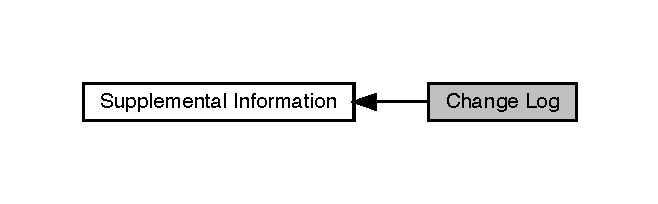
\includegraphics[width=316pt]{a00847}
\end{center}
\end{figure}
